\documentclass[]{informeutn}

% Librerías adicionales de TikZ para diagramas de flujo y estados
\usetikzlibrary{shapes.geometric, arrows.meta, positioning, calc, backgrounds, fit}

\usepackage{csquotes}
\usepackage{attachfile}

% Unidades adicionales
\newcommand{\MHz}{\,\unit{\mega\hertz}}
\newcommand{\kHz}{\,\unit{\kilo\hertz}}

% Recurso bibliográfico
\addbibresource{fuentes.bib}

% Configuración del paquete listings para código fuente
\definecolor{codegreen}{rgb}{0,0.55,0}
\definecolor{codegray}{rgb}{0.45,0.45,0.45}
\definecolor{codepurple}{rgb}{0.55,0,0.80}
\definecolor{codebg}{rgb}{0.97,0.97,0.97}

\lstdefinestyle{codestyle}{
  backgroundcolor=\color{codebg},
  basicstyle=\scriptsize\ttfamily,
  breakatwhitespace=false,
  breaklines=true,
  captionpos=b,
  commentstyle=\color{codegreen},
  frame=single,
  keepspaces=true,
  keywordstyle=\color{blue}\bfseries,
  numbers=left,
  numbersep=6pt,
  numberstyle=\tiny\color{codegray},
  rulecolor=\color{black!30},
  showspaces=false,
  showstringspaces=false,
  showtabs=false,
  stepnumber=1,
  stringstyle=\color{codepurple},
  tabsize=2,
  extendedchars=true,
  literate=
    {á}{{\'a}}1 {é}{{\'e}}1 {í}{{\'i}}1 {ó}{{\'o}}1 {ú}{{\'u}}1
    {Á}{{\'A}}1 {É}{{\'E}}1 {Í}{{\'I}}1 {Ó}{{\'O}}1 {Ú}{{\'U}}1
    {ñ}{{\~n}}1 {Ñ}{{\~N}}1
    {¿}{{?`}}1 {¡}{{!`}}1
    {•}{{$\bullet$}}1 {±}{{$\pm$}}1 {≥}{{$\ge$}}1 {—}{{---}}1
    {°}{{$^\circ$}}1
    {☀}{{[sol]}}1 {☀️}{{[sol]}}1
    {⚠}{{[aviso]}}1 {⚠️}{{[aviso]}}1
    {✔️}{{[ok]}}1 {✔}{{[ok]}}1
    {🌙}{{[luna]}}1
    {🔥}{{[fuego]}}1
}

% Metadatos del informe
\materia{Técnicas Digitales II -- Hackathon 2026}
\titulo{Central Semafórica de Dos Fases}
\subtitulo{Firmware Multitarea en FreeRTOS sobre STM32 y Aplicación Modbus RTU Maestro}
\comision{4R2}
\autores{Gastón Grasso 401892\\ Franco Palombo 401910\\ Angelo Prieto 401012}
\fecha{\today}

\begin{document}

  \maketitle
  \tableofcontents
  \setcounter{page}{1}
  \thispagestyle{plain}

  \chapter{Introducción}
\label{sec:introduccion}

El presente informe detalla el desarrollo, la arquitectura de firmware y la aplicación de control para la central
electrónica de semáforos diseñada en el marco del Hackathon 2026. El propósito del proyecto consistió en concebir e
implementar un sistema capaz de regular el tránsito vehicular y peatonal en una intersección de dos fases
ortogonales (Norte--Sur y Este--Oeste).

El núcleo de control fue desarrollado sobre la plataforma embebida STM32F103 (Blue Pill), cuyo microcontrolador
ARM Cortex-M3 opera junto con el sistema operativo de tiempo real FreeRTOS. A partir de una arquitectura multitarea
desacoplada, el firmware gestiona la máquina de estados de las señales luminosas, ejecuta la adquisición periódica de
sensores y variables de diagnóstico, y atiende peticiones de comunicación serie industrial bajo el protocolo Modbus RTU
en modalidad esclavo.

De manera complementaria, se diseñó (con el uso de la IA) una aplicación de supervisión y comando que asume el rol de
maestro en la red.  Esta herramienta permite auditar en tiempo real la telemetría del controlador, conmutar modos de
operación en caliente y reprogramar los intervalos temporales de cada fase sin interrumpir la ejecución del sistema. En
los capítulos siguientes se expone detalladamente el funcionamiento interno del firmware, el esquema de estados y la
integración con la interfaz de usuario.

  \chapter{Arquitectura y Funcionamiento del Firmware}
\label{sec:firmware}

El firmware de la central semafórica se estructuró a partir de una separación funcional en tres tareas concurrentes
administradas por el núcleo FreeRTOS. La sincronización y el intercambio de información entre las tareas se realiza
a través de un vector global compartido en memoria RAM, el cual mapea directamente la tabla de registros Modbus RTU.
Este diseño desacopla el control temporal de las luces, la lectura periódica de transductores y la atención de la
interfaz serie.

\section{Inicialización del Hardware y Flujo de Ejecución}
\label{sec:hw_init}

Al energizarse la placa STM32F103, se actualiza la frecuencia del núcleo a $72\MHz$ mediante la función
\texttt{SystemCoreClockUpdate}. Seguidamente, la rutina \texttt{vHardwareInit} habilita los relojes de periféricos
en el bus APB2 (puertos GPIOA, GPIOB, GPIOC, AFIO, USART1 y ADC1). Para maximizar la precisión del conversor analógico
a digital sin exceder el límite operativo de $14\MHz$, se configuró el prescaler del ADC en factor DIV6 ($12\MHz$).

A fin de utilizar el pin PB4 como salida de control para la lámpara roja de la Fase 1, se modificó el registro
\texttt{AFIO->MAPR} para deshabilitar la función JTAG y conservar el depurador SWD activo. Las salidas destinadas a
los cabezales luminosos se configuraron en modo push-pull con límite de velocidad de $2\MHz$: PB4 (Rojo), PB5
(Amarillo) y PB6 (Verde) para la Fase 1 (Norte--Sur); PB7 (Rojo), PB8 (Amarillo) y PB9 (Verde) para la Fase 2
(Este--Oeste). El pin PC13, vinculado al led integrado de la placa, se declaró como salida para proporcionar una señal
visual de actividad en cada conmutación.

\begin{figure}[!ht]
  \centering
  \resizebox{\textwidth}{!}{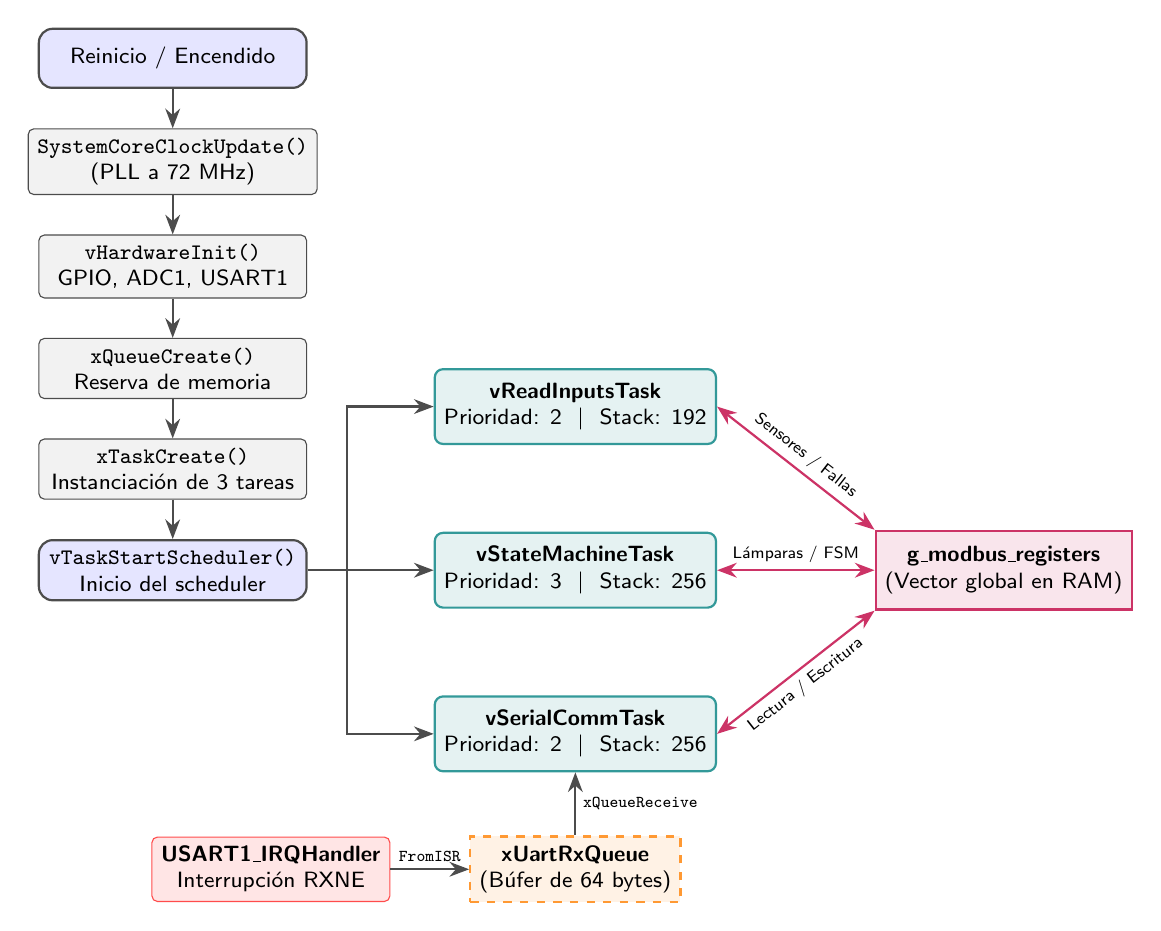
\begin{tikzpicture}[
    auto,
    font = \footnotesize\sffamily,
    node distance = 0.8cm and 1.2cm,
    startstop/.style = {rectangle, rounded corners=5pt, minimum width=3.4cm, minimum height=0.75cm, align=center, draw=black!70, fill=blue!10, thick},
    process/.style = {rectangle, minimum width=3.4cm, minimum height=0.75cm, align=center, draw=black!70, fill=gray!10, rounded corners=2pt},
    task/.style = {rectangle, minimum width=3.2cm, minimum height=0.95cm, align=center, draw=teal!80, fill=teal!10, rounded corners=3pt, thick},
    queue/.style = {rectangle, minimum width=2.4cm, minimum height=0.75cm, align=center, draw=orange!80, fill=orange!10, dashed, thick},
    shared/.style = {rectangle, minimum width=3.2cm, minimum height=1.0cm, align=center, draw=purple!80, fill=purple!10, thick},
    isr/.style = {rectangle, minimum width=2.6cm, minimum height=0.75cm, align=center, draw=red!70, fill=red!10, rounded corners=2pt},
    arrow/.style = {-{Stealth[length=2.5mm]}, thick, draw=black!70},
    darrow/.style = {{Stealth[length=2.5mm]}-{Stealth[length=2.5mm]}, thick, draw=purple!80}
]

  % Columna 1: Inicialización secuencial del sistema
  \node (start) [startstop] {Reinicio / Encendido};
  \node (clock) [process, below=0.5cm of start] {\texttt{SystemCoreClockUpdate()}\\(PLL a 72 MHz)};
  \node (hwinit) [process, below=0.5cm of clock] {\texttt{vHardwareInit()}\\GPIO, ADC1, USART1};
  \node (init_res) [process, below=0.5cm of hwinit] {\texttt{xQueueCreate()}\\Reserva de memoria};
  \node (tasks) [process, below=0.5cm of init_res] {\texttt{xTaskCreate()}\\Instanciación de 3 tareas};
  \node (sched) [startstop, below=0.5cm of tasks] {\texttt{vTaskStartScheduler()}\\Inicio del scheduler};

  \draw [arrow] (start) -- (clock);
  \draw [arrow] (clock) -- (hwinit);
  \draw [arrow] (hwinit) -- (init_res);
  \draw [arrow] (init_res) -- (tasks);
  \draw [arrow] (tasks) -- (sched);

  % Columna 2: Tareas concurrentes bajo FreeRTOS
  \node (t_fsm) [task, right=1.6cm of sched] {\textbf{vStateMachineTask}\\Prioridad: 3 \ \textbar\ \ Stack: 256};
  \node (t_io)  [task, above=1.1cm of t_fsm] {\textbf{vReadInputsTask}\\Prioridad: 2 \ \textbar\ \ Stack: 192};
  \node (t_ser) [task, below=1.1cm of t_fsm] {\textbf{vSerialCommTask}\\Prioridad: 2 \ \textbar\ \ Stack: 256};

  \draw [arrow] (sched.east) -- ++(0.5,0) |- (t_fsm.west);
  \draw [arrow] (sched.east) -- ++(0.5,0) |- (t_io.west);
  \draw [arrow] (sched.east) -- ++(0.5,0) |- (t_ser.west);

  % Columna 3: Vector global compartido en RAM
  \node (reg) [shared, right=2.0cm of t_fsm] {\textbf{g\_modbus\_registers}\\(Vector global en RAM)};

  \draw [darrow] (t_fsm.east) -- node [above, scale=0.75] {Lámparas / FSM} (reg.west);
  \draw [darrow] (t_io.east)  -- node [above, scale=0.75, sloped] {Sensores / Fallas} (reg.north west);
  \draw [darrow] (t_ser.east) -- node [below, scale=0.75, sloped] {Lectura / Escritura} (reg.south west);

  % Cadena de recepción serie (ISR -> Cola -> Tarea Serial) limpia sin cruzar líneas
  \node (queue) [queue, below=0.8cm of t_ser] {\textbf{xUartRxQueue}\\(Búfer de 64 bytes)};
  \node (isr)   [isr, left=1.0cm of queue] {\textbf{USART1\_IRQHandler}\\Interrupción RXNE};

  \draw [arrow] (isr.east) -- node [above, scale=0.75] {\texttt{FromISR}} (queue.west);
  \draw [arrow] (queue.north) -- node [right, scale=0.75] {\texttt{xQueueReceive}} (t_ser.south);

\end{tikzpicture}
}
  \caption{Flujo general de inicialización y arquitectura multitarea en FreeRTOS.}
  \label{fig:flujo_firmware}
\end{figure}

Para la adquisición de magnitudes analógicas, los terminales PB0 (canal 8 de ADC1) y PB1 (canal 9 de ADC1) se
dispusieron en modo analógico de alta impedancia, aplicando un tiempo de integración extendido de 239.5 ciclos de
reloj para minimizar la impedancia de entrada y el ruido. Por su parte, el periférico USART1 se ajustó a una velocidad
de $115200$ baudios con formato 8-N-1 sobre los pines PA9 (TX) y PA10 (RX). Se habilitó la interrupción por registro de
recepcion no vacío (\texttt{RXNEIE}).

Antes de transferir el control al scheduler, la función \texttt{main} reserva una cola de 64 bytes
(\texttt{xUartRxQueue}) para almacenar los caracteres recibidos por la interrupción serie, e instancia las tres tareas
principales detalladas en la figura~\ref{fig:flujo_firmware}.

\section{Tarea de Control de Fases y Lógica de Semáforos}
\label{sec:fsm_task}

La tarea \texttt{vStateMachineTask} ejecuta con prioridad 3, la más alta de la aplicación, garantizando que los
cambios de fase y los mecanismos de despeje no sufran demoras por tareas secundarias. Al iniciar la tarea, se adoptó
como criterio de diseño preventivo un arranque seguro en Estado 2 (Todo Rojo) durante $2\s$, permitiendo despejar
la intersección y estabilizar el sistema antes de iniciar la circulación.

\begin{figure}[!ht]
  \centering
  \resizebox{\textwidth}{!}{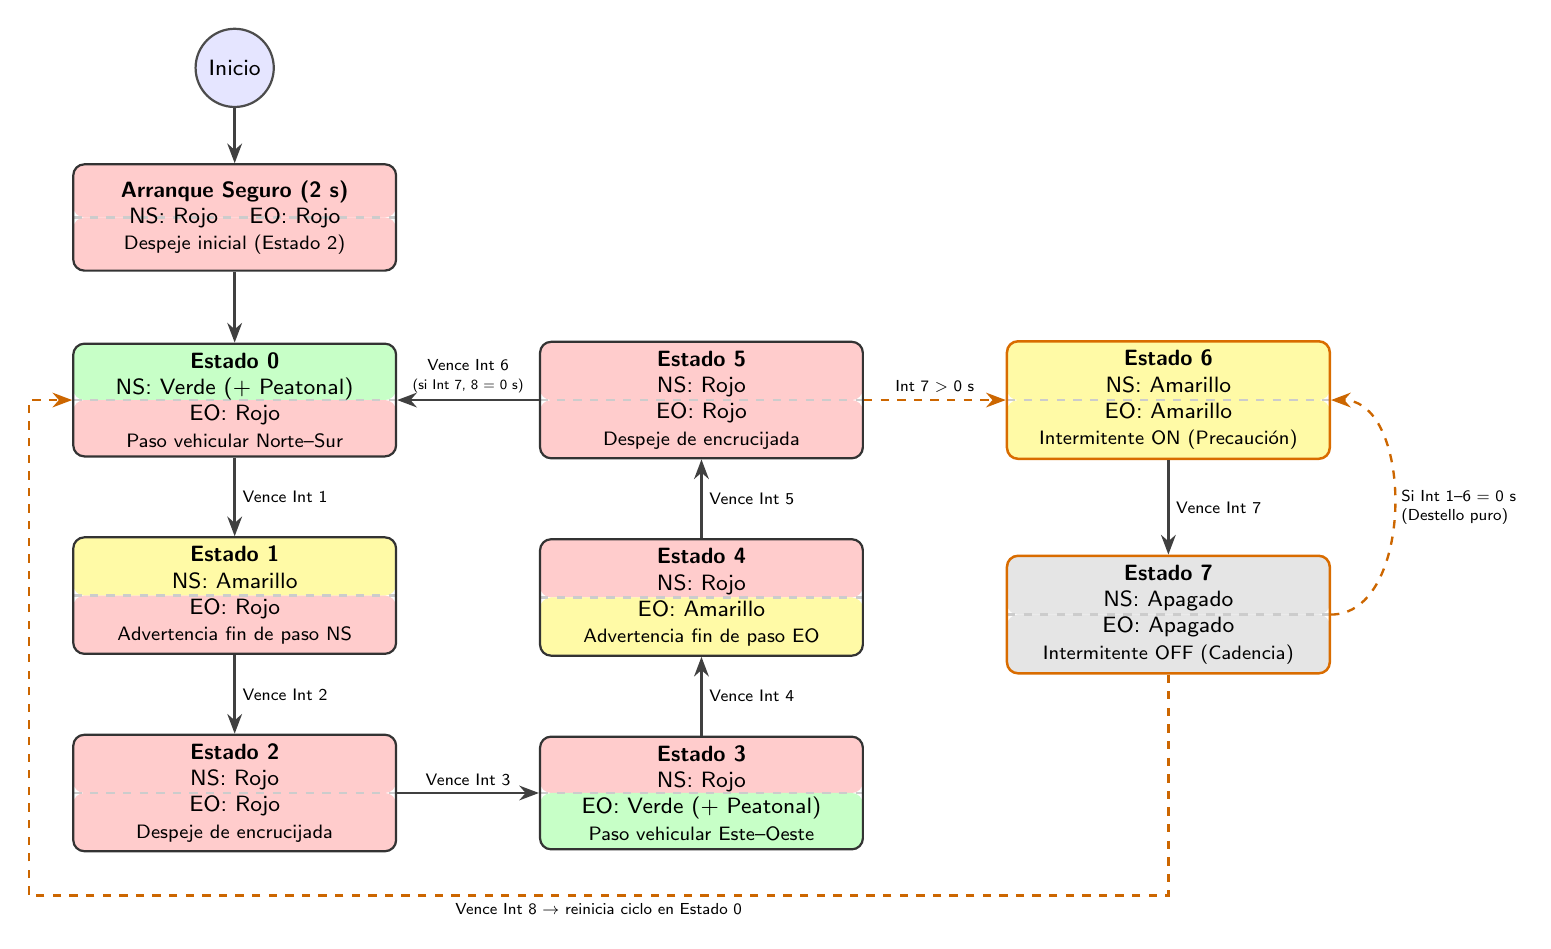
\begin{tikzpicture}[
    auto,
    font=\footnotesize\sffamily,
    node distance=1.1cm and 1.8cm,
    splitstate/.style 2 args={
      rectangle, rounded corners=4pt, minimum width=4.1cm, minimum height=1.35cm,
      align=center, draw=black!80, line width=0.8pt,
      path picture={
        \fill[#1] (path picture bounding box.north west) rectangle (path picture bounding box.east);
        \fill[#2] (path picture bounding box.west) rectangle (path picture bounding box.south east);
        \draw[black!20, dashed] (path picture bounding box.west) -- (path picture bounding box.east);
      }
    },
    intermitstate/.style 2 args={
      rectangle, rounded corners=4pt, minimum width=4.1cm, minimum height=1.35cm,
      align=center, draw=orange!85!black, line width=0.9pt,
      path picture={
        \fill[#1] (path picture bounding box.north west) rectangle (path picture bounding box.east);
        \fill[#2] (path picture bounding box.west) rectangle (path picture bounding box.south east);
        \draw[black!20, dashed] (path picture bounding box.west) -- (path picture bounding box.east);
      }
    },
    startnode/.style={circle, minimum size=0.85cm, align=center, draw=black!70, fill=blue!10, thick},
    arrow/.style={-{Stealth[length=2.5mm]}, line width=0.9pt, draw=black!75},
    cfgarrow/.style={-{Stealth[length=2.5mm]}, line width=0.85pt, draw=orange!80!black, dashed}
]

  % Nodo de Inicio y Arranque Seguro
  \node (start) [startnode] {Inicio};
  
  \node (boot) [splitstate={red!20}{red!20}, below=0.7cm of start] {
    \textbf{Arranque Seguro (2 s)}\\
    NS: Rojo \quad EO: Rojo\\
    \scriptsize Despeje inicial (Estado 2)
  };

  % Columna 1 (Izquierda): Fase 1 (Norte-Sur vehicular activa)
  \node (st0) [splitstate={green!22}{red!20}, below=0.9cm of boot] {
    \textbf{Estado 0}\\
    NS: Verde (+ Peatonal)\\
    EO: Rojo\\
    \scriptsize Paso vehicular Norte--Sur
  };

  \node (st1) [splitstate={yellow!35}{red!20}, below=1.0cm of st0] {
    \textbf{Estado 1}\\
    NS: Amarillo\\
    EO: Rojo\\
    \scriptsize Advertencia fin de paso NS
  };

  \node (st2) [splitstate={red!20}{red!20}, below=1.0cm of st1] {
    \textbf{Estado 2}\\
    NS: Rojo\\
    EO: Rojo\\
    \scriptsize Despeje de encrucijada
  };

  % Columna 2 (Centro): Fase 2 (Este-Oeste vehicular activa)
  \node (st3) [splitstate={red!20}{green!22}, right=1.8cm of st2] {
    \textbf{Estado 3}\\
    NS: Rojo\\
    EO: Verde (+ Peatonal)\\
    \scriptsize Paso vehicular Este--Oeste
  };

  \node (st4) [splitstate={red!20}{yellow!35}, above=1.0cm of st3] {
    \textbf{Estado 4}\\
    NS: Rojo\\
    EO: Amarillo\\
    \scriptsize Advertencia fin de paso EO
  };

  \node (st5) [splitstate={red!20}{red!20}, above=1.0cm of st4] {
    \textbf{Estado 5}\\
    NS: Rojo\\
    EO: Rojo\\
    \scriptsize Despeje de encrucijada
  };

  % Columna 3 (Derecha): Régimen Intermitente / Destellante (Estados 6 y 7)
  \node (st6) [intermitstate={yellow!35}{yellow!35}, right=1.8cm of st5] {
    \textbf{Estado 6}\\
    NS: Amarillo\\
    EO: Amarillo\\
    \scriptsize Intermitente ON (Precaución)
  };

  \node (st7) [intermitstate={black!10}{black!10}, below=1.2cm of st6] {
    \textbf{Estado 7}\\
    NS: Apagado\\
    EO: Apagado\\
    \scriptsize Intermitente OFF (Cadencia)
  };

  % Conexiones del flujo de arranque y ciclo vehicular
  \draw [arrow] (start) -- (boot);
  \draw [arrow] (boot) -- (st0);
  \draw [arrow] (st0) -- node [right, scale=0.75] {Vence Int 1} (st1);
  \draw [arrow] (st1) -- node [right, scale=0.75] {Vence Int 2} (st2);
  \draw [arrow] (st2) -- node [above, scale=0.75] {Vence Int 3} (st3);
  \draw [arrow] (st3) -- node [right, scale=0.75] {Vence Int 4} (st4);
  \draw [arrow] (st4) -- node [right, scale=0.75] {Vence Int 5} (st5);

  % Retorno directo del ciclo vehicular cuando Int 7 = 0 y Int 8 = 0
  \draw [arrow] (st5.west) -- node [above, scale=0.72, align=center] {Vence Int 6\\{\scriptsize (si Int 7, 8 = 0 s)}} (st0.east);

  % Conexión hacia Estados 6 y 7 cuando Int 7 > 0 s
  \draw [cfgarrow] (st5.east) -- node [above, scale=0.72, align=center] {Int 7 $>$ 0 s} (st6.west);
  \draw [arrow] (st6) -- node [right, scale=0.75] {Vence Int 7} (st7);

  % Retorno desde Estado 7 al inicio del ciclo (perimetral inferior) o lazo intermitente
  \coordinate (under) at ($(st2.south)+(0,-0.55cm)$);
  \draw [cfgarrow] (st7.south) -- (st7.south |- under) 
    -- node [below, scale=0.72] {Vence Int 8 $\to$ reinicia ciclo en Estado 0}
    ($(st0.west |- under)+(-0.55cm,0)$) 
    -- ($(st0.west)+(-0.55cm,0)$) -- (st0.west);
  \draw [cfgarrow] (st7.east) to[out=0, in=0] node [right, scale=0.72, align=left] {Si Int 1--6 = 0 s\\(Destello puro)} (st6.east);

\end{tikzpicture}
}
  \caption{Diagrama de transiciones de la máquina de estados cíclica de 8 intervalos.}
  \label{fig:fsm_semaforo}
\end{figure}

Superada la etapa de arranque, la tarea opera sobre un anillo cíclico unificado de 8 intervalos temporales
configurables (Estados 0 al 7), ilustrado en la figura~\ref{fig:fsm_semaforo}:
\begin{itemize}
  \item \texttt{Estado 0:} Habilita el paso vehicular en sentido Norte--Sur, manteniendo la fase Este--Oeste detenida.
  \item \texttt{Estado 1:} Transición de advertencia en Norte--Sur con luz amarilla activa y Este--Oeste
    en rojo.
  \item \texttt{Estado 2:} Intervalo de despeje de encrucijada con ambas fases en Todo Rojo.
  \item \texttt{Estado 3:} Habilita el paso vehicular en sentido Este--Oeste, manteniendo la fase Norte--Sur detenida.
  \item \texttt{Estado 4:} Transición de advertencia en Este--Oeste con luz amarilla activa y Norte--Sur
    en rojo.
  \item \texttt{Estado 5:} Segundo intervalo de despeje de encrucijada en Todo Rojo.
  \item \texttt{Estado 6:} Régimen intermitente encendido con lámparas amarillas activas en ambas fases.
  \item \texttt{Estado 7:} Régimen intermitente apagado con todas las lámparas desconectadas.
\end{itemize}

El funcionamiento se rige directamente por la tabla de duraciones almacenada en los registros Modbus
\texttt{REG\_TIME\_INT1} a \texttt{REG\_TIME\_INT8}. En cada iteración, la tarea evalúa la duración del estado
correspondiente:
\begin{itemize}
  \item Si la duración es mayor a cero ($t > 0$), se actualiza el registro \texttt{REG\_FSM\_STATE}, se
    asientan las máscaras de lámparas en \texttt{REG\_LIGHTS\_NS} y \texttt{REG\_LIGHTS\_EO}, y se comutan las salidas de
    hardware mediante \texttt{vHardwareSetLights}. La espera temporal se ejecuta segundo a segundo con
    \texttt{vTaskDelay(pdMS\_TO\_TICKS(1000))}; en cada segundo se examina si el registro fue puesto en cero por el
    maestro, permitiendo truncar o acelerar la transición en caliente sin latencias residuales.
  \item Si la duración es nula ($t = 0\s$), el estado se omite de forma instantánea sin demora, avanzando el índice
    hacia el siguiente intervalo del anillo.
\end{itemize}

Esta arquitectura unificada y gobernada por tabla elimina la necesidad de bifurcaciones asíncronas o modos forzados
rígidos: en el régimen vehicular ordinario, los Estados 6 y 7 se configuran con duración $0\s$, recorriéndose
exclusivamente los Estados 0 al 5. Por el contrario, para establecer un régimen intermitente de precaución (en horario
nocturno o ante mantenimiento), basta con reprogramar en cero los intervalos 1 al 6 y asignar la cadencia deseada a los
intervalos 7 y 8 (por ejemplo, $1\s$ activo y $1\s$ inactivo), logrando la conmutación de forma fluida y determinística.

\section{Tarea de Adquisición de Transductores y Diagnóstico}
\label{sec:inputs_task}

La tarea \texttt{vReadInputsTask} se ejecuta con prioridad 2 y periodicidad estricta de $100\ms$ mediante la función
\texttt{vTaskDelayUntil}, eliminando derivas temporales en la adquisición de señales. En cada ciclo operativo se
desarrollan cuatro procesos de medición y diagnóstico:

En primer lugar, se adquiere la tensión del divisor resistivo vinculado al LDR en el pin PB0. Con el propósito de
atenuar fluctuaciones por ruido de conmutación, la tarea promedia cuatro conversiones consecutivas y transforma el valor
crudo de 12 bits a milivoltios. Dicho valor se almacena en el registro \texttt{REG\_LDR\_MV} y se evalúa frente al
parámetro \texttt{REG\_LDR\_THRESHOLD\_MV} (fijado por defecto en $2000\mV$). Si la lectura supera este umbral, se
activa el bit de detección nocturna en el registro de entradas digitales (\texttt{INPUT\_LDR\_NIGHT}).

En segundo lugar, se muestrea el pin PB1, en el cual se conectó un potenciómetro que emula la corriente total consumida
por las lámparas del semáforo en un rango de $0$ a $1200\mA$.

En tercer lugar, se evalúa la presencia de la red eléctrica primaria y se estima el nivel de tensión de la batería de
respaldo en el registro \texttt{REG\_BATTERY\_MV}. En ausencia de suministro de red, el algoritmo simula la descarga
progresiva de la batería; al descender la tensión por debajo de $11.0\V$, se asienta la alarma correspondiente en el
registro de fallas.

Por último, el firmware calcula la corriente total que teóricamente deberían drenar los cabezales luminosos en base
al número de lámparas activas en ambas fases:
\begin{equation}
  I_{\mathrm{esperada}} = N_{\mathrm{activas}} \cdot I_{\mathrm{nominal}}
  \label{eq:corriente_esperada}
\end{equation}
donde $I_{\mathrm{nominal}}$ se encuentra definido en \texttt{REG\_LAMP\_CURRENT\_MA}. Sobre este valor se determina una
banda admisible de corriente aplicando la tolerancia porcentual estipulada en \texttt{REG\_CURRENT\_TOL\_PCT}:
\begin{gather}
  I_{\mathrm{min}} = I_{\mathrm{esperada}} \cdot \left(1 - \frac{\mathrm{Tol}\%}{100}\right) \nonumber \\
  I_{\mathrm{max}} = I_{\mathrm{esperada}} \cdot \left(1 + \frac{\mathrm{Tol}\%}{100}\right)
  \label{eq:banda_tolerancia}
\end{gather}

Si la corriente medida en PB1 resulta inferior a $I_{\mathrm{min}}$ habiendo lámparas encendidas, el sistema asume
la desconexión o rotura de filamentos y levanta la bandera de lámpara quemada (\texttt{FAULT\_LAMP\_BURNED}). Por el
contrario, si supera $I_{\mathrm{max}}$, se reporta un evento de sobrecorriente o cortocircuito
(\texttt{FAULT\_OVERCURRENT}). De esta forma, la central electrónica efectúa un monitoreo en tiempo real del estado de
los emisores luminosos.

\section{Tarea de Comunicaciones Serie y Protocolo Modbus RTU}
\label{sec:modbus_task}

La atención de las comunicaciones reside en la tarea \texttt{vSerialCommTask}, configurada con prioridad 2. La
recepción física de datos se gestiona mediante la rutina de interrupción \texttt{USART1\_IRQHandler}. Cuando el
registro de recepción contiene un byte nuevo (\texttt{RXNE}), este se introduce en la cola \texttt{xUartRxQueue}
utilizando la función no bloqueante \texttt{xQueueSendFromISR}.

Para estructurar las tramas sin recurrir a sondeos que degraden el rendimiento de la CPU, la tarea adopta una lógica
de espera dual: cuando el búfer de recepción se encuentra vacío, la tarea se bloquea por tiempo indefinido
(\texttt{portMAX\_DELAY}), asegurando un consumo de procesamiento nulo. Una vez ingresado el primer carácter, el tiempo
máximo de espera en cola se ajusta a $5\ms$. Este valor satisface holgadamente el criterio de silencio entre tramas
$t_{3.5}$ estipulado en la norma Modbus RTU para velocidades superiores a $19200$ baudios. Cuando el temporizador
vence sin que ingresen nuevos caracteres, se da por finalizada la trama y se procede a su decodificación.

El paquete se somete al cálculo del código de redundancia cíclica de 16 bits (CRC16) con el polinomio reflejado
$0\mathrm{xA001}$. Si el código coincide con el recibido y el primer byte concuerda con la dirección asignada a la
central (\texttt{MODBUS\_SLAVE\_ID = 1}), se ejecuta la función \texttt{vModbusProcessFrame}, la cual procesa dos
códigos de función estándar:
\begin{itemize}
  \item \texttt{Función 0x03 (Read Holding Registers):} Extrae un bloque contiguo de variables del vector global
  \texttt{g\_modbus\_registers}, armando el mensaje de respuesta con el conteo de bytes y su correspondiente CRC.
  \item \texttt{Función 0x06 (Write Single Register):} Permite al maestro modificar en caliente un registro de
  configuración (como las duraciones de los intervalos temporales o los umbrales de diagnóstico). La respuesta
  consiste en el eco exacto de la trama recibida.
\end{itemize}

\section{Mapa de Registros Modbus RTU}
\label{sec:mapa_modbus}

En la tabla~\ref{tab:mapa_modbus} se detalla la distribución de variables en el vector global compartido,
especificando las direcciones lógicas, el significado de cada registro y los valores nominales cargados durante la
fase de arranque.

\begin{table}[!ht]
  \centering
  \small
  \renewcommand{\arraystretch}{1.18}
  \caption{Mapa de registros Modbus RTU implementado en el firmware de la central.}
  \label{tab:mapa_modbus}
  \begin{tabular}{c l c c p{6.5cm}}
    \toprule
    \textbf{Reg.} & \textbf{Nombre Simbólico} & \textbf{Acceso} & \textbf{Valor} & \textbf{Descripción} \\
    \midrule
    0 & \texttt{REG\_TIME\_INT1} & R/W & $25\s$ & Duración Intervalo 1: NS Verde / EO Rojo \\
    1 & \texttt{REG\_TIME\_INT2} & R/W & $3\s$  & Duración Intervalo 2: NS Amarillo / EO Rojo \\
    2 & \texttt{REG\_TIME\_INT3} & R/W & $2\s$  & Duración Intervalo 3: Despeje Todo Rojo \\
    3 & \texttt{REG\_TIME\_INT4} & R/W & $25\s$ & Duración Intervalo 4: NS Rojo / EO Verde \\
    4 & \texttt{REG\_TIME\_INT5} & R/W & $3\s$  & Duración Intervalo 5: NS Rojo / EO Amarillo \\
    5 & \texttt{REG\_TIME\_INT6} & R/W & $2\s$  & Duración Intervalo 6: Despeje Todo Rojo \\
    6 & \texttt{REG\_TIME\_INT7} & R/W & $0\s$  & Duración Intervalo 7: Intermitente ON (Amarillos) \\
    7 & \texttt{REG\_TIME\_INT8} & R/W & $0\s$  & Duración Intervalo 8: Intermitente OFF (Apagados) \\
    8 & \texttt{REG\_FSM\_STATE} & R   & 0      & Estado activo de la máquina de estados (0 a 7) \\
    9 & \texttt{REG\_LIGHTS\_NS} & R   & 0      & Luces Norte--Sur [B0:R, B1:A, B2:V, B3:Peat] \\
    10 & \texttt{REG\_LIGHTS\_EO} & R  & 0      & Luces Este--Oeste [B0:R, B1:A, B2:V, B3:Peat] \\
    11 & \texttt{REG\_BATTERY\_MV} & R & $12600\mV$ & Tensión estimada de batería de respaldo \\
    12 & \texttt{REG\_CURRENT\_MA} & R & $0\mA$     & Corriente total medida por transductor \\
    13 & \texttt{REG\_INPUTS\_DIGITAL} & R & 1   & Entradas [B0: Red 220V, B1: Noche LDR] \\
    14 & \texttt{REG\_FAULT\_FLAGS} & R    & 0   & Fallas [B0: Lámpara, B1: Bat baja, B2: Imax] \\
    15 & \texttt{REG\_LDR\_MV} & R         & $500\mV$ & Tensión analógica leída en sensor LDR \\
    16 & \texttt{REG\_LDR\_THRESHOLD\_MV} & R/W & $2000\mV$ & Umbral de conmutación crepuscular \\
    17 & \texttt{REG\_LAMP\_CURRENT\_MA} & R/W & $200\mA$ & Corriente nominal por lámpara activa \\
    18 & \texttt{REG\_CURRENT\_TOL\_PCT} & R/W & $35\%$   & Tolerancia de corriente admisible \\
    19 & \texttt{REG\_EXPECTED\_CURR\_MA} & R  & $400\mA$ & Corriente calculada según luces activas \\
    \bottomrule
  \end{tabular}
\end{table}

  \chapter{Aplicación de Control y Supervisión (Maestro Modbus)}
\label{sec:aplicacion_control}

Para la verificación funcional  de la central semafórica, se diseñó con el uso de la IA una aplicación de
supervisión que asume el rol de equipo Maestro en la red de comunicaciones. La herramienta fue desarrollada
utilizando tecnologías web (HTML5, CSS y JavaScript) y aprovecha la interfaz Web Serial API para comunicarse de
forma bidireccional con el puerto serie físico del microcontrolador STM32F103 a una velocidad de $115200$ baudios
con trama 8-N-1.

\begin{figure}[!ht]
  \centering
  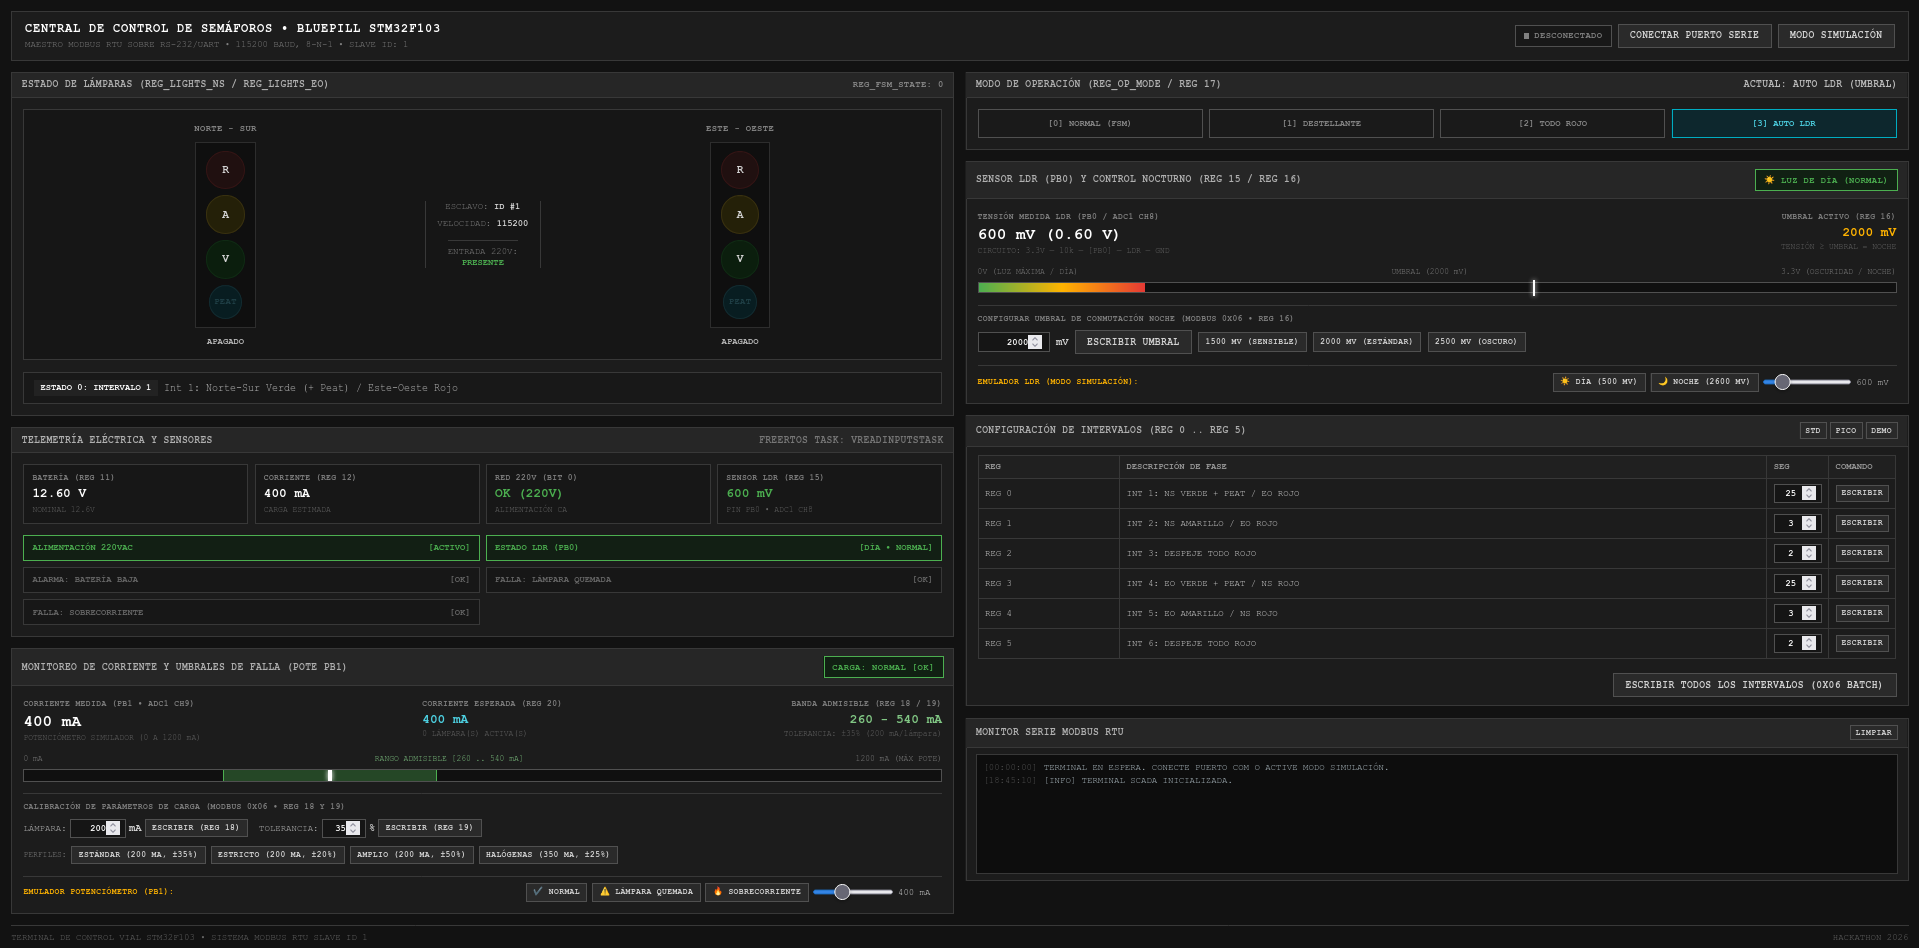
\includegraphics[width=\textwidth]{images/interfaz_maestro.png}
  \caption{Panel de supervisión y control maestro desarrollado para la central semafórica.}
  \label{fig:interfaz_maestro}
\end{figure}

Como se aprecia en la captura de la figura~\ref{fig:interfaz_maestro}, la interfaz de usuario se distribuye en paneles
especializados que reflejan en tiempo real el contenido del vector de registros del esclavo:
\begin{enumerate}
  \item \texttt{Estado de Lámparas y Cabezales:} Presenta la representación gráfica de las dos fases (Norte--Sur y
  Este--Oeste), reproduciendo el encendido de los discos luminoso vehicular (Rojo, Amarillo y Verde) y de la flecha
  peatonal. Este bloque se refresca mediante la lectura periódica de los registros \texttt{REG\_LIGHTS\_NS} y
  \texttt{REG\_LIGHTS\_EO}.
  \item \texttt{Telemetría Eléctrica y Banderas de Alarma:} Informa la tensión estimada de la batería de respaldo, la
  corriente total consumida, la presencia de la red eléctrica primaria de $220\V$ y el estado del sensor crepuscular.
  Asimismo, expone los indicadores de falla por sobrecorriente, lámpara quemada o batería baja.
  \item \texttt{Monitoreo de Corriente y Umbrales:} Incluye un indicador de barra horizontal que contrasta la corriente
  medida frente a la ventana de tolerancia admisible calculada por el microcontrolador. En la interfaz es posible
  ajustar el valor nominal de cada lámpara ($200\mA$ por defecto) y el porcentaje de tolerancia ($\pm 35\%$),
  escribiendo sobre los registros 17 y 18 (\texttt{REG\_LAMP\_CURRENT\_MA} y \texttt{REG\_CURRENT\_TOL\_PCT}).
  \item \texttt{Preajustes y Calibración Nocturna:} Ofrece selectores de régimen operativo para cargar en
  caliente conjuntos de intervalos (Ciclo Normal, Destellante o Despeje) y un control para calibrar el umbral
  crepuscular en milivoltios mediante el registro 16 (\texttt{REG\_LDR\_THRESHOLD\_MV}).
  \item \texttt{Configuración de Intervalos Temporales:} Dispone de campos de edición numérica para los registros 0 a 7,
  permitiendo reprogramar en caliente las duraciones de cada fase vehicular y despeje (Intervalos 1 a 6), así como la
  cadencia de los estados intermitentes (Intervalos 7 y 8) mediante tramas de escritura Modbus (función 0x06).
  \item \texttt{Monitor de Tráfico Serie:} Consola inferior que registra los paquetes transmitidos y recibidos,
  permitiendo constatar la integridad del protocolo y el cómputo de CRC16.
\end{enumerate}

La herramienta no solo facilitó las pruebas de laboratorio en banco, sino que también demostró la viabilidad de
integrar la central local dentro de un esquema de telecontrol urbano centralizado.

  \chapter{Conclusiones}
\label{sec:conclusiones}

El desarrollo y verificación del firmware sobre el microcontrolador STM32F103 (núcleo ARM Cortex-M3) junto con el
sistema operativo FreeRTOS permitieron cumplir satisfactoriamente con los requerimientos operativos planteados para el
Hackathon 2026.
La división funcional en tres tareas concurrentes con prioridades diferenciadas demostró ser eficaz para desacoplar
las responsabilidades críticas de control temporal frente a los procesos de diagnóstico analógico y comunicación
serie.

En particular, la estrategia de arranque seguro con retardo de despeje en Todo Rojo y el submuestreo temporal en
bloques de $100\ms$ dentro de la máquina de estados garantizaron una respuesta inmediata ante cambios de modo o
consignas recibidas por la red serie, evitando estados intermedios inconsistentes o demoras perjudiciales en la
señalización vial. Asimismo, la incorporación del algoritmo de cálculo de corriente esperada posibilitó la detección
precoz de anomalías por lámparas abiertas o sobrecorrientes en los cabezales, confiriendo al equipo capacidades de
diagnóstico preventivo.

Por su parte, la implementación del protocolo estándar Modbus RTU sobre la interfaz USART1, asistida por una cola de
interrupción y detección de fin de trama por silencio de línea ($t_{3.5}$), aseguró una comunicación confiable con el
panel de supervisión web sin sobrecargar la CPU. En definitiva, la solución técnica alcanzada combina robustez en la
conmutación física de fases, flexibilidad de configuración remota y supervisión activa del estado del sistema.


  \nocite{*}
  \printbibliography[heading=bibnumbered, title={Fuentes}]

  \chapter{Anexos: Archivos Fuente y Recursos Adjuntos}
\label{sec:anexos}

Con el propósito de mantener la concisión del documento y facilitar la inspección directa del código, los archivos
fuente del proyecto se han incorporado como adjuntos embebidos en este documento PDF.

Los lectores de documentos PDF compatibles (tales como Adobe Acrobat Reader, Okular, Evince o los visores integrados
de navegadores modernos) permiten extraer, guardar y visualizar directamente los archivos haciendo clic sobre las
anotaciones de la tabla~\ref{tab:anexos_adjuntos} o accediendo al panel lateral de archivos adjuntos del visor.

\begin{table}[!ht]
  \centering
  \small
  \caption{Listado de archivos fuente y recursos técnicos embebidos en el documento.}
  \label{tab:anexos_adjuntos}
  \begin{tabular}{c l p{6.4cm} c}
    \toprule
    \textbf{Elemento} & \textbf{Archivo} & \textbf{Descripción Técnica} & \textbf{Adjunto} \\
    \midrule
    1 & \texttt{modbus\_registers.h} & Definición del mapa de registros y máscaras de bits & \attachfile[description={Archivo de cabecera modbus-registers.h}]{sources/include/modbus_registers.h} \\
    2 & \texttt{main.c} & Firmware de la central en FreeRTOS sobre STM32F103 & \attachfile[description={Codigo fuente principal main.c}]{sources/src/main.c} \\
    3 & \texttt{FreeRTOSConfig.h} & Configuración del núcleo de tiempo real FreeRTOS & \attachfile[description={Configuracion FreeRTOS}]{sources/include/FreeRTOSConfig.h} \\
    4 & \texttt{index.html} & Aplicación web SCADA y Maestro Modbus RTU & \attachfile[description={Aplicacion web index.html}]{sources/index.html} \\
    \bottomrule
  \end{tabular}
\end{table}

\section{Estructura de los Recursos Adjuntos}
\label{sec:descripcion_recursos}

A continuación se resume el alcance de cada uno de los archivos embebidos:
\begin{itemize}
  \item \texttt{modbus\_registers.h:} Cabecera en lenguaje C que tipifica los 20 registros del vector global compartido,
  las constantes de tiempo predeterminadas y las banderas de diagnóstico vial.
  \item \texttt{main.c:} Implementación completa del firmware embebido, comprendiendo la inicialización de hardware, el
  manejador de interrupciones de USART1, la máquina de estados (\texttt{vStateMachineTask}), el muestreo analógico
  (\texttt{vReadInputsTask}) y el procesador de comandos Modbus (\texttt{vSerialCommTask}).
  \item \texttt{index.html:} Aplicación autónoma desarrollada en HTML5, CSS y JavaScript que implementa la lógica de
  maestro Modbus RTU, comunicándose con el hardware mediante la interfaz Web Serial API o en modo de simulación.
  \item \texttt{FreeRTOSConfig.h:} Parámetros del planificador apropiativo, configuración de la frecuencia del tick a
  $1\unit{\kilo\hertz}$, asignación de memoria heap y prioridades de interrupción de FreeRTOS.
\end{itemize}


\end{document}
